
\documentclass[paper=a4, parskip, fontsize=11pt]{scrartcl}
\usepackage[left= 2cm, right = 2cm, bottom = 2cm, top = 4cm]{geometry}
\setlength{\parindent}{0em} 
\title{cs-opt optimization report}
\author{cs-opt}
\date{\today}

\makeatletter
\let\newtitle\@title
\let\newauthor\@author
\let\newdate\@date
\makeatother

\usepackage[hyphens]{url}
\usepackage[
pdfsubject={},
pdfauthor={cs-opt},
pdfkeywords={},
%Links nicht einrahmen
hidelinks
]{hyperref}

% Packages
\usepackage{amsmath}
\usepackage{amsfonts}
\usepackage[onehalfspacing]{setspace}
\usepackage[utf8]{inputenc}
\usepackage[T1]{fontenc}
\usepackage{lmodern}
\usepackage{graphicx}
\usepackage{subcaption}
\graphicspath{{img/}}
\usepackage[headsepline=true, markcase=upper]{scrlayer-scrpage}
\usepackage{booktabs}
\usepackage{tabularx}
% \usepackage[ngerman]{babel}
\usepackage[english]{babel}
\usepackage{caption}
\usepackage{relsize}
\usepackage{placeins}
\usepackage{chngcntr}
\usepackage{longtable}
\usepackage{bm}
\usepackage[short]{optidef}

% Header
\lohead{\today}
\rohead{\includegraphics[height=35pt]{DLR_logo.png}}
\cohead{Institute of Vehicle Concepts}

% align at the top of the page
\makeatletter
\setlength{\@fptop}{0pt}
\setlength{\@fpbot}{0pt plus 1fil}
\makeatother

\cofoot[]{}


\pagenumbering{roman}

% Document
\begin{document}
	

	
    \begin{center}
        \LARGE{\textsc{cs-opt optimization report}}
    \end{center}
    %\vspace*{5px}
    This report summarizes the canonical form of the investigated optimization problem and its results.
    %\vspace*{5px}
    \begin{mini*}
    {x}{\text{Specific Absorpion Eenrgy} \rightarrow \bm{f(x)}}{}{} 
    \addConstraint{\text{Total Vehicle mass} \rightarrow \bm{g_1(x)}}{\leq 0}
    \addConstraint{\text{intrusion: 5266147 in [mm]} \rightarrow \bm{g_2(x)}}{\leq 0}
    \addConstraint{\text{intrusion: 5266147 in [mm]} \rightarrow \bm{g_3(x)}}{\leq 0}
    \addConstraint{\text{intrusion: 5266147 in [mm]} \rightarrow \bm{g_4(x)}}{\geq -2.7}
    \addConstraint{\text{intrusion: 5266147 in [mm]} \rightarrow \bm{g_9(x)}}{\leq 0}
    \addConstraint{\text{intrusion: 5266147 in [mm]} \rightarrow \bm{g_{10}(x)}}{\geq 3.0}
    \addConstraint{t_{BU}}{\in C_{t_{BU}} = [0.0-5.0]}
    \addConstraint{x_{1}}{\in C_1 = [0.0-5.0]}
    \addConstraint{x_{1}}{\in C_1 = [0.0-5.0]}
    \addConstraint{x_{1}}{\in C_1 = [0.0-5.0]}
    \addConstraint{x_{1}}{\in C_1 = [0.0-5.0]}
	\addConstraint{x_{2}}{\in D_2 = [1000,2000,3000,1000,2000,3000]}
    \addConstraint{x_{2}}{\in D_2 = [1000,2000,3000]} 
    \addConstraint{x_{2}}{\in D_2 = [1000,2000,3000]} 
    \addConstraint{x_{2}}{\in D_2 = [1000,2000,3000]} 
    \addConstraint{x_{2}}{\in D_2 = [1000,2000,3000]}
    \end{mini*}


    The following optimizations settings have been used to run the optimization.
	\vspace*{10px}
	\begin{table}[hbt!]
		\renewcommand{\arraystretch}{1.5}
		\begin{tabular}{llllr}
			\textbf{epsilon: }        &  1.2345 & {   }  & \textbf{encoding: }   &  1.2345  \\
			\textbf{parallel jobs:}      &  1743547 & {   } & \textbf{use SCIP: }          &  -320.75 \\
			\textbf{CV:}                 &  732946 & {   } & \textbf{stop if feasible:}   &  -320.75 \\
			\textbf{max time SCIP:}      &  57.96 & {   } & \textbf{SCIP gap: }          &  -320.75 \\
			\textbf{max time Grad:}      &  -1049.87 & {   } & \textbf{modify constraints:} &  -320.75 \\
			\textbf{CV error metric:}    &  -887.68 & {   } & \textbf{modify constraints:} &  -320.75 \\
			\textbf{Metamodels: }        &  -320.75 & {   } & \textbf{modification value:} &  -320.75 \\
			\textbf{Scale response: }    &  -1049.87 & {   } & \textbf{use Localsearch: }   &  -320.75 \\
		\end{tabular}
		\renewcommand{\arraystretch}{1}
	\end{table}

	The convergence trend is shown in the figure below. The red points represent the designs where one or more constraints have been violated. Green ones represent designs that satisfy all constraints functions. The yellow marker identifies the optimal solution. 

    
    \begin{figure}[hbt!]
	% include first image
	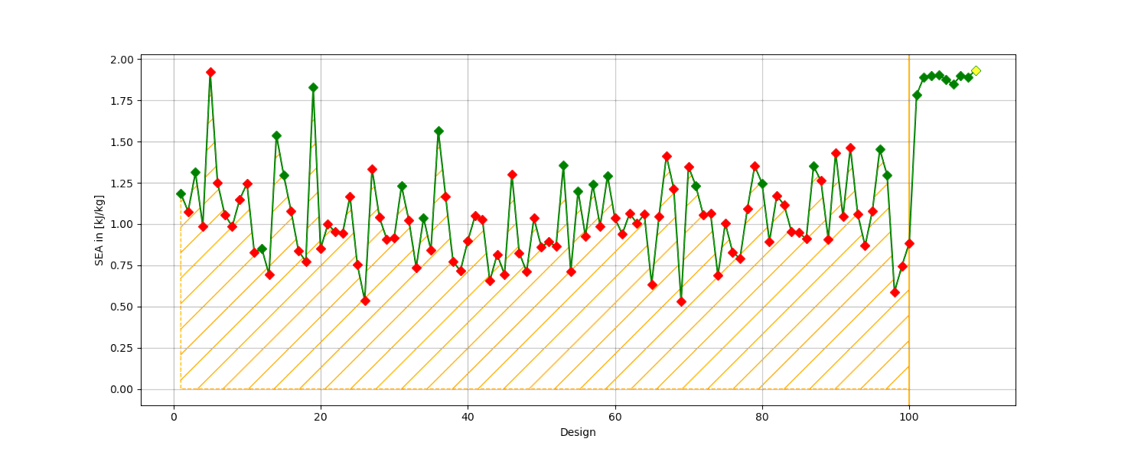
\includegraphics[width=1.0\linewidth]{convergence_Opti5.png}
	\caption{Convergence History Curve}
	\label{fig:convergence}
	\end{figure}
    
    Every iteration steps is summarized in the table below.
    

    % here comes the table of results
    \begin{center}
    	\begin{longtable}{lrrrrrrrrrrrrr} % add one column
    		
    		\caption{Table of Results} 
    		\label{tab:long}  \\
    		\hline 
    		\multicolumn{1}{r}{\textbf{}} &  
    		\multicolumn{1}{r}{\textbf{x1}} & 
    		\multicolumn{1}{r}{\textbf{x2}} & 
    		\multicolumn{1}{r}{\textbf{x3}} &
    		\multicolumn{1}{r}{\textbf{x4}} &
    		\multicolumn{1}{r}{\textbf{x5}} &
    		\multicolumn{1}{r}{\textbf{x6}} &
    		\multicolumn{1}{r}{\textbf{x7}} &
    		\multicolumn{1}{r}{\textbf{x8}} &
    		\multicolumn{1}{r}{\textbf{x9}} &
    		\multicolumn{1}{r}{\textbf{x10}}& 
    		\multicolumn{1}{r}{\textbf{x11}}&
    		\multicolumn{1}{r}{\textbf{f(x)}}&
    		\multicolumn{1}{r}{\textbf{g(x)}}
    		
    		\\ \hline 
    		\endfirsthead
    		
    		\multicolumn{14}{c} %set the number of columns here  
    		{{ \tablename\ \thetable{: Table of Results}}} \\
    		\hline 
    		\multicolumn{1}{r}{\textbf{}} & 
    		\multicolumn{1}{r}{\textbf{x1}} & 
    		\multicolumn{1}{r}{\textbf{x2}} &
    		\multicolumn{1}{r}{\textbf{x3}} &
    		\multicolumn{1}{r}{\textbf{x4}} &
    		\multicolumn{1}{r}{\textbf{x5}} &
    		\multicolumn{1}{r}{\textbf{x6}} &
    		\multicolumn{1}{r}{\textbf{x7}} &
    		\multicolumn{1}{r}{\textbf{x8}} &
    		\multicolumn{1}{r}{\textbf{x9}} &
    		\multicolumn{1}{r}{\textbf{x10}}&
    		\multicolumn{1}{r}{\textbf{x11}}&
			\multicolumn{1}{r}{\textbf{f(x)}}&
			\multicolumn{1}{r}{\textbf{g(x)}}
    		\\ \hline 
    		\endhead
    		
    		\hline %\multicolumn{3}{|r|}{{Continued on next page}} \\ \hline
    		\endfoot
    		
    		\hline %\hline
    		\endlastfoot
    		
    		0001 &    1.570 &    3.180 & 1.890 &    1.110 &    1.510 &    1.540 &    1.070 &   3000  & 1000 &  20000000 & 3000 & 0.234 & 24.23 \\
    		0002 &    1.570 &    3.180 & 1.890 &    1.110 &    1.510 &    1.540 &    1.070 &   3000  & 1000 &  20000000 & 3000 & 0.234 & 24.23 \\
    		0003 &    1.570 &    3.180 & 1.890 &    1.110 &    1.510 &    1.540 &    1.070 &   3000  & 1000 &  20000000 & 3000 & 0.234 & 24.23 \\
    		0004 &    1.570 &    3.180 & 1.890 &    1.110 &    1.510 &    1.540 &    1.070 &   3000  & 1000 &  20000000 & 3000 & 0.234 & 24.23 \\
    		0005 &    1.570 &    3.180 & 1.890 &    1.110 &    1.510 &    1.540 &    1.070 &   3000  & 1000 &  20000000 & 3000 & 0.234 & 24.23 \\
    		0006 &    1.570 &    3.180 & 1.890 &    1.110 &    1.510 &    1.540 &    1.070 &   3000  & 1000 &  20000000 & 3000 & 0.234 & 24.23 \\
    		0007 &    1.570 &    3.180 & 1.890 &    1.110 &    1.510 &    1.540 &    1.070 &   3000  & 1000 &  20000000 & 3000 & 0.234 & 24.23 \\
    		0008 &    1.570 &    3.180 & 1.890 &    1.110 &    1.510 &    1.540 &    1.070 &   3000  & 1000 &  20000000 & 3000 & 0.234 & 24.23 \\
    		0009 &    1.570 &    3.180 & 1.890 &    1.110 &    1.510 &    1.540 &    1.070 &   3000  & 1000 &  20000000 & 3000 & 0.234 & 24.23 \\
    		0010 &    1.570 &    3.180 & 1.890 &    1.110 &    1.510 &    1.540 &    1.070 &   3000  & 1000 &  20000000 & 3000 & 0.234 & 24.23 \\
    		0011 &    1.570 &    3.180 & 1.890 &    1.110 &    1.510 &    1.540 &    1.070 &   3000  & 1000 &  20000000 & 3000 & 0.234 & 24.23 \\
    		0012 &    1.570 &    3.180 & 1.890 &    1.110 &    1.510 &    1.540 &    1.070 &   3000  & 1000 &  20000000 & 3000 & 0.234 & 24.23 \\
    		0013 &    1.570 &    3.180 & 1.890 &    1.110 &    1.510 &    1.540 &    1.070 &   3000  & 1000 &  20000000 & 3000 & 0.234 & 24.23 \\
    		0001 &    1.570 &    3.180 & 1.890 &    1.110 &    1.510 &    1.540 &    1.070 &   3000  & 1000 &  20000000 & 3000 & 0.234 & 24.23 \\
    		0001 &    1.570 &    3.180 & 1.890 &    1.110 &    1.510 &    1.540 &    1.070 &   3000  & 1000 &  20000000 & 3000 & 0.234 & 24.23 \\
    		0001 &    1.570 &    3.180 & 1.890 &    1.110 &    1.510 &    1.540 &    1.070 &   3000  & 1000 &  20000000 & 3000 & 0.234 & 24.23 \\
    		0001 &    1.570 &    3.180 & 1.890 &    1.110 &    1.510 &    1.540 &    1.070 &   3000  & 1000 &  20000000 & 3000 & 0.234 & 24.23 \\
    		0001 &    1.570 &    3.180 & 1.890 &    1.110 &    1.510 &    1.540 &    1.070 &   3000  & 1000 &  20000000 & 3000 & 0.234 & 24.23 \\
    		0001 &    1.570 &    3.180 & 1.890 &    1.110 &    1.510 &    1.540 &    1.070 &   3000  & 1000 &  20000000 & 3000 & 0.234 & 24.23 \\
    		0001 &    1.570 &    3.180 & 1.890 &    1.110 &    1.510 &    1.540 &    1.070 &   3000  & 1000 &  20000000 & 3000 & 0.234 & 24.23 \\
    		0001 &    1.570 &    3.180 & 1.890 &    1.110 &    1.510 &    1.540 &    1.070 &   3000  & 1000 &  20000000 & 3000 & 0.234 & 24.23 \\
    		0001 &    1.570 &    3.180 & 1.890 &    1.110 &    1.510 &    1.540 &    1.070 &   3000  & 1000 &  20000000 & 3000 & 0.234 & 24.23 \\
    		0001 &    1.570 &    3.180 & 1.890 &    1.110 &    1.510 &    1.540 &    1.070 &   3000  & 1000 &  20000000 & 3000 & 0.234 & 24.23 \\
    		0001 &    1.570 &    3.180 & 1.890 &    1.110 &    1.510 &    1.540 &    1.070 &   3000  & 1000 &  20000000 & 3000 & 0.234 & 24.23 \\
    		0001 &    1.570 &    3.180 & 1.890 &    1.110 &    1.510 &    1.540 &    1.070 &   3000  & 1000 &  20000000 & 3000 & 0.234 & 24.23 \\
    	\end{longtable}
    \end{center}

The initial design was improved about 13\% while fullfilling all the chosen constraints.
\vspace*{10px}
\begin{table}[hbt!]
	\centering
	\begin{tabular}{p{0.10\textwidth}>{\raggedleft}p{0.2\textwidth}>{\raggedleft\arraybackslash}p{0.2\textwidth}}
		\toprule
		\textbf{}   &   \textbf{Initial Design}      & \textbf{Best Design}   \\
		\midrule
		\textbf{f(x)}       &         0.05  & 1.23  \\
		\textbf{g(x)}       &       983.05029 &    183.15137 \\
		\textbf{x1}  &  746   & 123       \\
		\textbf{x2}  &  746   & 123       \\
		\textbf{x3}  &  746   & 123       \\
		\textbf{x4}  &  746   & 123       \\
		\textbf{x5}  &  746   & 123       \\
		\textbf{x6}  &  746   & 123       \\
		\textbf{x7}  &  746   & 123       \\
		\textbf{x8}  &  746   & 123       \\
		\textbf{x9}  &  746   & 123       \\
		\textbf{x10}  &  746   & 123       \\
		\textbf{x11}  &  746   & 123       \\
		\bottomrule
	\end{tabular}
	\caption{Comparison of the starting Design and the optimized Design}
	\label{tab:tab1}
\end{table}


\begin{figure}[hbt!]
	% include first image
	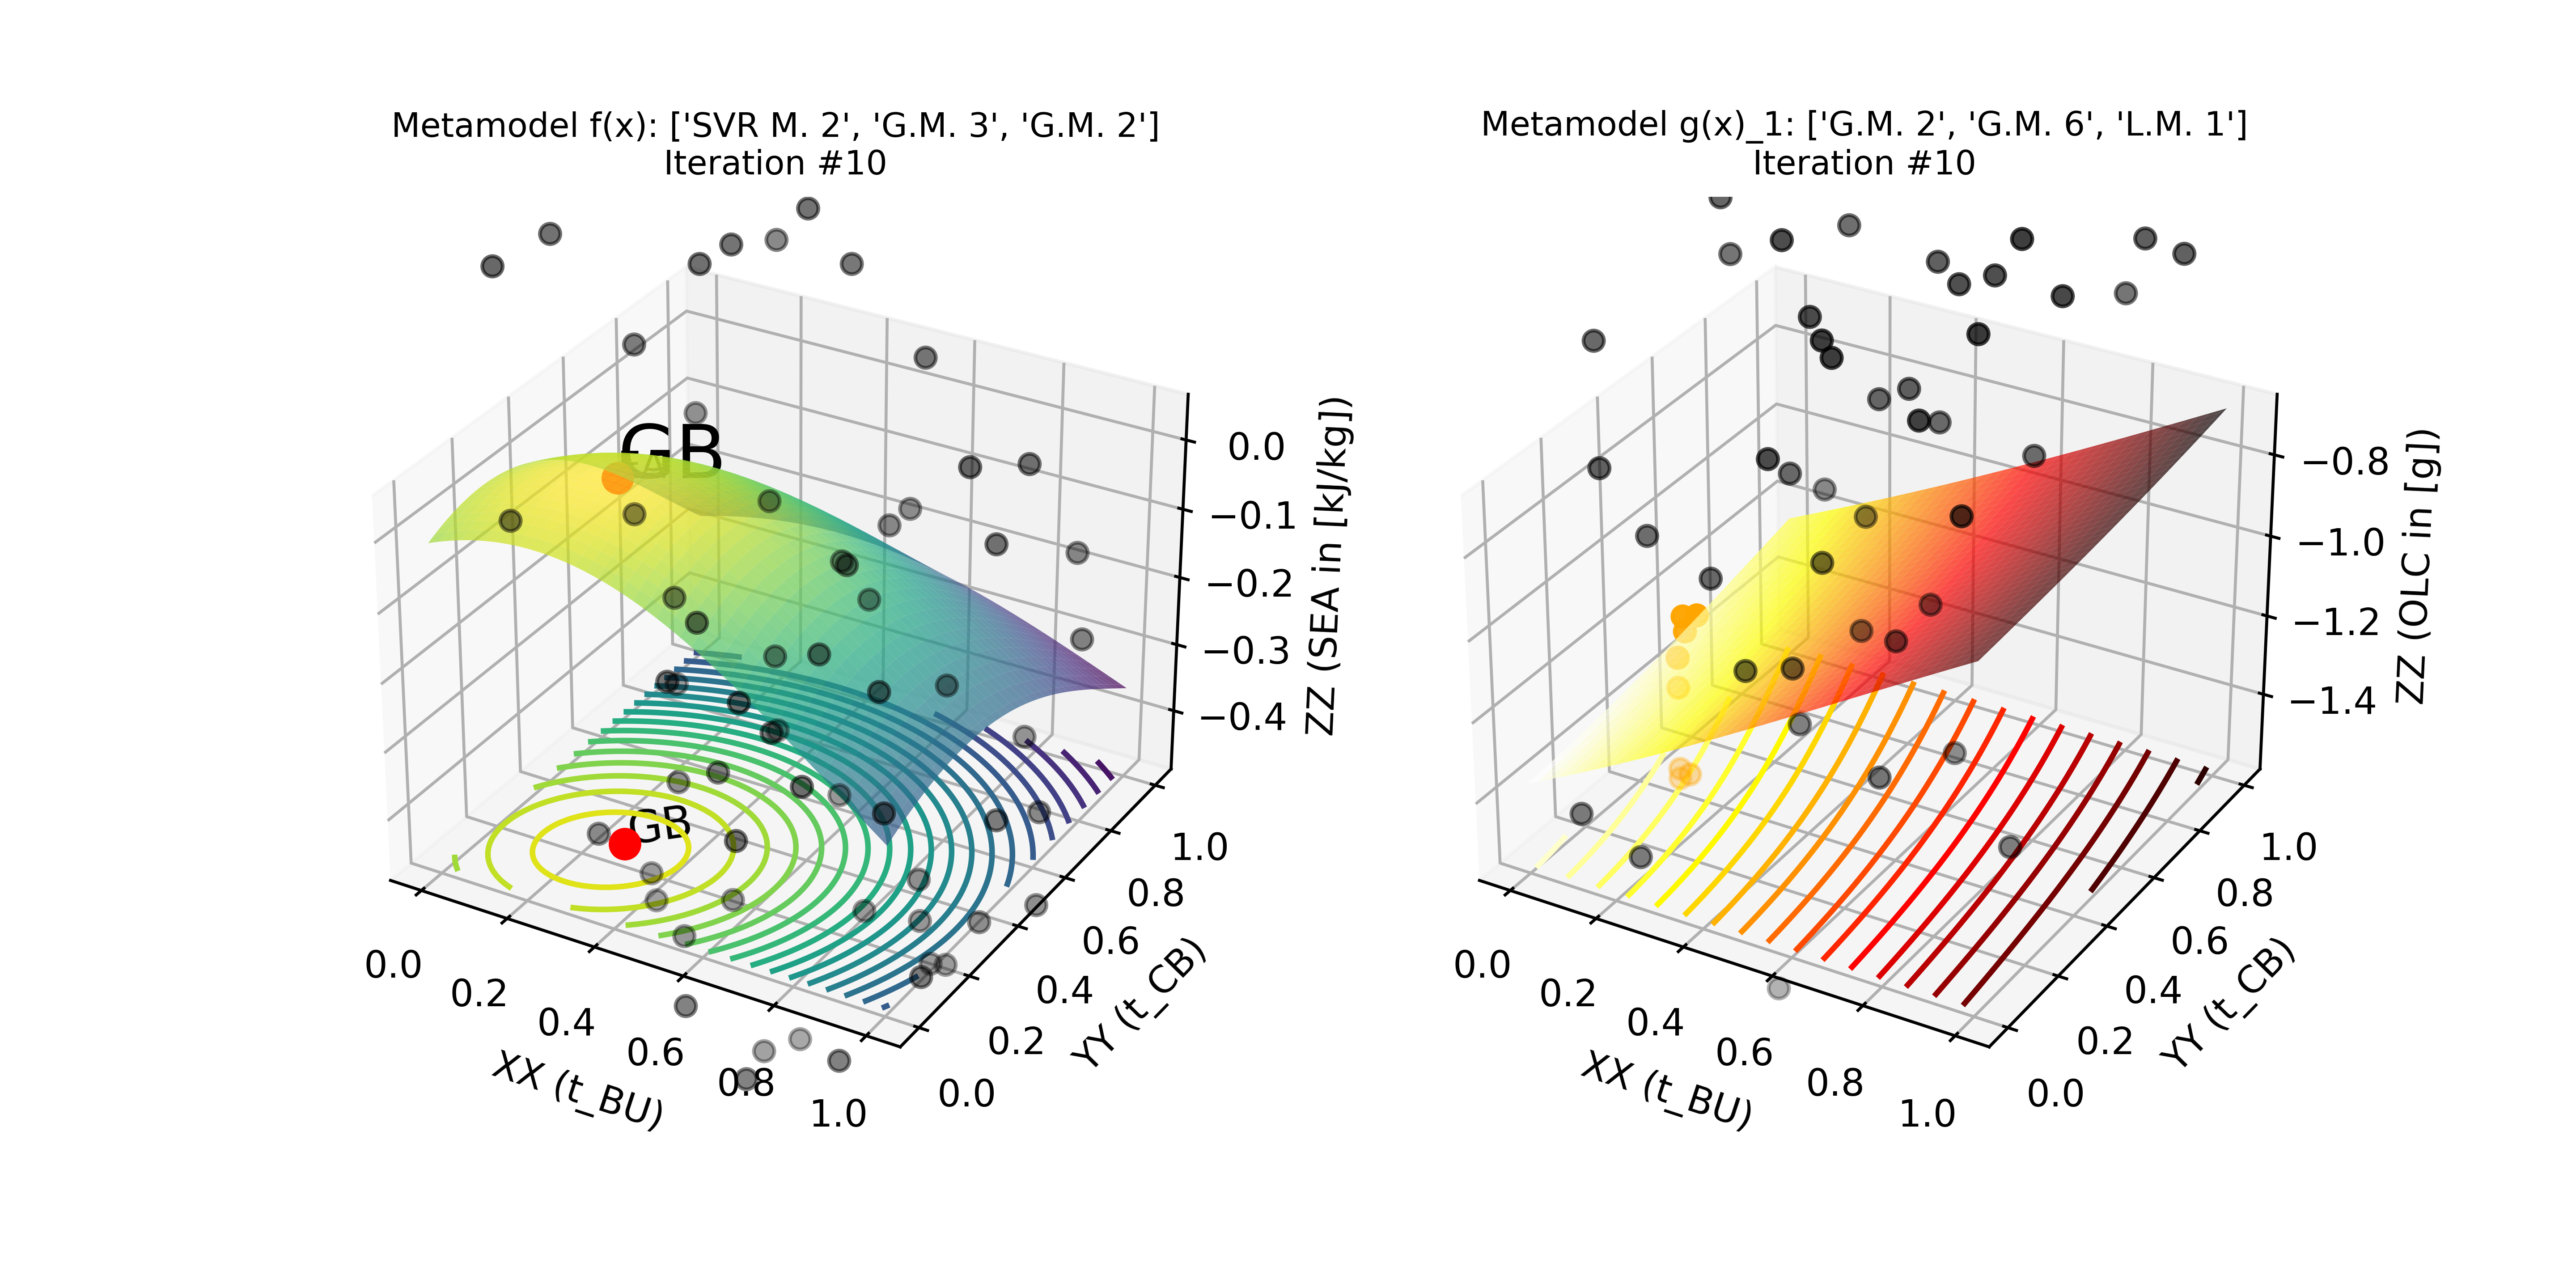
\includegraphics[width=1.0\linewidth]{Metamodel10t_BU_vs_t_CB.png}
	\caption{Metamodels of the Optimal Design}
	\label{fig:metamodel}
\end{figure}

%Metamodel10t_BU_vs_t_CB.png

\end{document}

